%%% template.tex
%%%
%%% This LaTeX source document can be used as the basis for your technical
%%% paper or abstract. Intentionally stripped of annotation, the parameters
%%% and commands should be adjusted for your particular paper - title, 
%%% author, article DOI, etc.
%%% The accompanying ``template.annotated.tex'' provides copious annotation
%%% for the commands and parameters found in the source document. (The code
%%% is identical in ``template.tex'' and ``template.annotated.tex.'')

\documentclass[annual]{acmsiggraph}


\TOGonlineid{45678}
\TOGvolume{0}
\TOGnumber{0}
\TOGarticleDOI{1111111.2222222}
\TOGprojectURL{}
\TOGvideoURL{}
\TOGdataURL{}
\TOGcodeURL{}

\usepackage{caption}
\usepackage{subcaption}
\usepackage[english]{babel}
\usepackage{hyperref}
\title{Spec2Fab: A  Graph-Based Framework for Fabricating Fabrication Algorithms}

\author{}
\pdfauthor{}

\keywords{}

\newcommand{\note}[1]{\marginpar{\LARGE $\spadesuit$}
			$\spadesuit$ {\bf #1} $\spadesuit$}

\begin{document}

 \teaser{
   \begin{subfigure}[b]{0.3\textwidth}
	\centering
    	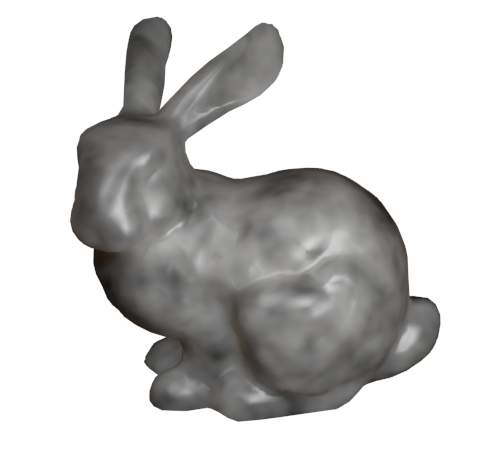
\includegraphics[width=0.6\textwidth]{figure/bunny_orig.png}
      	\caption{}
        \label{teaser:original}
        \end{subfigure}
        ~ 
        \begin{subfigure}[b]{0.18\textwidth}
                \centering
    	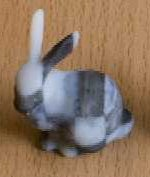
\includegraphics[width=\textwidth]{figure/bunny_print1.jpg}
                \caption{}
                \label{teaser:ours}
        \end{subfigure}
        ~
        \begin{subfigure}[b]{0.2\textwidth}
                \centering
    	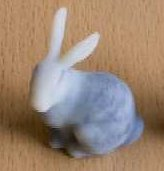
\includegraphics[width=\textwidth]{figure/bunny_print2.jpg}
                \caption{}
                \label{teaser:makerbot}
        \end{subfigure}
        ~
        \begin{subfigure}[b]{0.18\textwidth}
                \centering
    	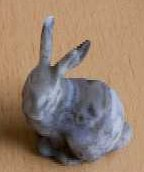
\includegraphics[width=\textwidth]{figure/bunny_print3.jpg}
                \caption{}
                \label{teaser:objet}
        \end{subfigure}
        \caption{A textured mesh printed with different types of 3D printers.
        	(a)original model.(b)printed with our printer.(c)makerbot.
        	(d)objet}\label{teaser}
	\label{fig:texture}
 }

\maketitle

\begin{abstract}


\end{abstract}

\keywordlist

\TOGlinkslist

\copyrightspace

\note{Teaser should be all different results produced using spec2Fab, texture, subsurface scattering, caustics etc...}


\section{Introduction}
Computational fabrication couples new digital manufacturing techniques with novel numerical algorithms to produce objects with remarkable physical characteristics. These methods are of great interest in computer graphics for two reasons: First, they provide us with  new class of output devices which can render into  real-life and second, they yield valuable insight into the accuracy of our numerical models of the world.  

In this paper we focus on a fundamental problem in producing any such custom object:  optimal material assignment. Given an object one must find a spatially varying material distribution that satisfies some given criteria. The algorithms that solve these problems are often complicated to develop, implement, test and modify. We provide a new graph-based framework which decomposes such problems into a small set of constituent components alleviating the above issues as well as facilitating the development and testing of new algorithms. 

\section{Related Work} 
Here we will review previous algorithms for solving the optimal material assignment problem . We divide this review into two broad categories, optimizing for desired optical properties and optimizing for desired mechanical properties. Finally we will briefly review work done on modular shader languages as they have influenced our current work.

Optimizing and manufacturing objects with desired optical characteristics is a popular problem in computer graphics. Building objects which embed image in their caustics has been explored by Finch \textit{et al.} ~\shortcite{Finckh:2010} and Papas \textit{et al.}\shortcite{Marios:2011}. Optimization based approaches have also been employed to control the subsurface scattering of printed 3D models ~\cite{Hasan:2010}. These approaches have also been extended to optically decrypt hidden images ~\cite{Papas:2012}. Finally, optimal shadow casting surfaces have been produced which emulate a given set of input images ~\cite{Bermano:2012}.

Fabricating objects with desired deformation characteristics has been explored less in the literature. Some recent examples include simulating and manufacturing layered composites ~\cite{Bickel:2010} as well as the design and construction of balloons with a desired shape while inflated ~\cite{sko:2012}. Finally, material optimization has been employed to create mechanical clones of human faces ~\cite{Bickel:2012}.

\autoref{tb:algorithms} shows the coordinate reduction method as well as the optimization scheme used in all cited works. A motivating observation for this research is that, despite different applications, these previous works share, not only a common methodology, but a set of common reduced coordinate components. These, in conjunction with (often off-the-shelf) optimization techniques form new material assignment algorithms. This suggests that one could find a small set of components that can be tied together to synthesize existing and new methods. Similar approaches have already proven useful for creating complex texture shading examples ~\cite{Cook1984}. Our goal in this paper is to produce an analogous mechanism for material assignment problems. 
\begin{table*}[htp]
\centering
\caption{The goal type, reduction type and optimization used by previous fabrication works.}
\begin{tabular}{clll}
\hline
\textbf{Paper} & \textbf{Goal} & \textbf{Reduced Coordinates}  & \textbf{Optimization} \\ 
\hline
~\cite{Bickel:2010}& Deformation & Layered Materials  & Branch and Bound \\
~\cite{Finckh:2010} & Optical (Caustics) & B-Spline Surface & SPSA \\
~\cite{Hasan:2010}& Optical (Subsurface) & Layered Materials & Branch and Bound\\ 
~\cite{Marios:2011} & Optical (Caustics) & Quadratic Surface Tiles & Simulated Annealing \\
~\cite{Bermano:2012} & Optical (Shadows) & Height Field & Custom/Simulated Annealing \\
~\cite{Bickel:2012} & Deformation &  Height Field &  Newton-Raphson \\
~\cite{Papas:2012} & Optical & Quadratic Surface Tiles & Simulated Annealing \\
~\cite{sko:2012}& Deformation & Triangle Mesh & ALM \\
\hline
\end{tabular}
\label{tb:algorithms}
\end{table*}
%\subsection{Simulation of the Appearance of Ink Combinations}
%\cite{Matusik:2009} built a system
%for the measurement of Bidirectional Reflectance Distribution Functions (BRDFs) and were able
%to acquire BRDFs for both single-layer and multi-layer ink printouts (e.g., an ink covered by a
%varnish layer). They then acquired a database of many different combinations of ink layers (up to
%seven layer combinations were considered). However, they did not develop a method to simulate
%the appearance of arbitrary ink layers. They were able to interpolate the appearance by spatially
%multiplexing small tiles of different base combinations. By linearity of light transport, the simulation
%of the combined appearance was reduced to linear combinations of the base BRDFs. 
%simulation method for the appearance of translucent materials \cite{Hasan:2010}. 
%They
%built a measurement system for estimating multiple-scattering in homogeneous material slabs. They
%measured both transmission and refection for a set of base materials used by the OBJET Connex
%multi-material printer. 
%Using these measurements, our simulations framework was able to predict
%diffuse reflections and transmissions in multi-layered translucent objects composed of base material
%layers.
%In the proposed research, we will extend these methods to cover the complete appearance of
%volumetric materials that accounts for both directly reflected light and light scattering within the
%material volume. 
%We will use efficient simulation methods that allows us to simulate the appearance
%of complex structures composed from these base materials. We developed an initial framework for
%simulating behavior of multi-layered materials, where each layer is a homogeneous base material.
%Then we extend this simulation to materials in which each voxel is made of a different measured
%material. Since this general simulation is expensive and requires path-tracing algorithms, we used
%algorithms that are based on fast numerical integration of our low-dimensional representations
%and the use of pre-computation, similar to pre-computed light transport approaches \cite{Sloan:2002}.
\section{Contributions}
The overall contribution of our work is a flexible framework for the construction of material assignment algorithms. Our second contribution is the ``Reducer Network'',  a graphical data structure which describes both the geometric partitioning and material parameterization of  a given object. We couple this with a ``Tuner Network'' which automatically tunes the parameters of the Reducer Network to produce a fabricable object. Finally we provide an extensible API which utilizes these structures to produce numerous material assignment algorithms from a set of primitive operations.
\section{Methods}
Below we will describe the key components of our framework and its associated API. We begin by describing the data structures that tie our framework together, the Reducer Network and the Tuner Network. We will then show how these two components interact to provide a compact graphical description of the material assignment problem. Finally we will show our basis set of components that we use to produce a wide-range of fabrication algorithms. 
\subsection{The Reducer Network}
Computing material assignments at output device resolution is computationally intractable. Because of this, material assignments are computed  using a reduced representation. We specify this representation using a Reducer Network.  This structure is conceptually similar to those used in programmable shading systems (e.g. ~\cite{Cook1984}, Maya Shader Networks) . However these systems are primarily concerned with assigning known materials and textures to an object's surface whereas we are seeking a volumetric assignment of (as yet) unknown materials. In order to accomplish this task we build a directed, acyclic graph which has the object's surface geometry as its root node. We define two classes of nodes, geometry nodes and parameterization nodes. A geometry node takes a volumetric region as input and produces a partition of unity of this region as output. The leaf nodes of our graph are the parameterization nodes which associate a material assignment function of the form $\lambda\left(x,y,z,\theta\right)$ to an input volumetric region. Lambda can either output material parameters or a discrete material assignment for a spatial point $\left(x,y,z\right)$ given some parameters, here denoted by $\theta$. Because the network describes a nested set of partitions of unity we can efficiently perform material queries by passing a query point through the network until it arrives at a parameterization node. We note that Reducer Networks do not inherently enforce material continuity between disjoint regions in the graph however, for material assignment problems this is neither required nor desired. 

 See \textbf{Figure 1} for an example of a Reducer Network. \note{Desai: Make figure 1}.  

\subsection{Tuners}
\note{Desai: can you write this section, I don't know the details}
\subsection{Tuning the Reducer Network}

\subsection{Tuner Network}
\note{Desai: also this section :) }
%\section{System Description}
%The software framework (shown in Figure~\ref{fig:framework}) is composed of 
%a set of software
%modules that can be easily modified or exchanged. The first component
%of this framework is an output-device-independent description API
%that allows the user to specify any physical object in terms of its physical
%properties such as geometry, mechanical behaviors, and appearance. 
%The framework will also provide physically-based
%simulation tools that accurately predict the behavior of our output device.
%The goal of the optimization module is to search through
%the space of possible device outputs and deliver one that best matches the
%desired model. In order to evaluate the quality of the match between the
%simulation output and the desired model we need to develop appropriate
%comparison metrics. Finally, a central component of our framework is
%a reduction model which makes the optimization problem tractable by
%reducing the search space as much as possible.
%The reduction model can specified by experts or deduced from a
%set of examples. Next, we will describe each element of the framework in
%more detail.
%\begin{figure}
%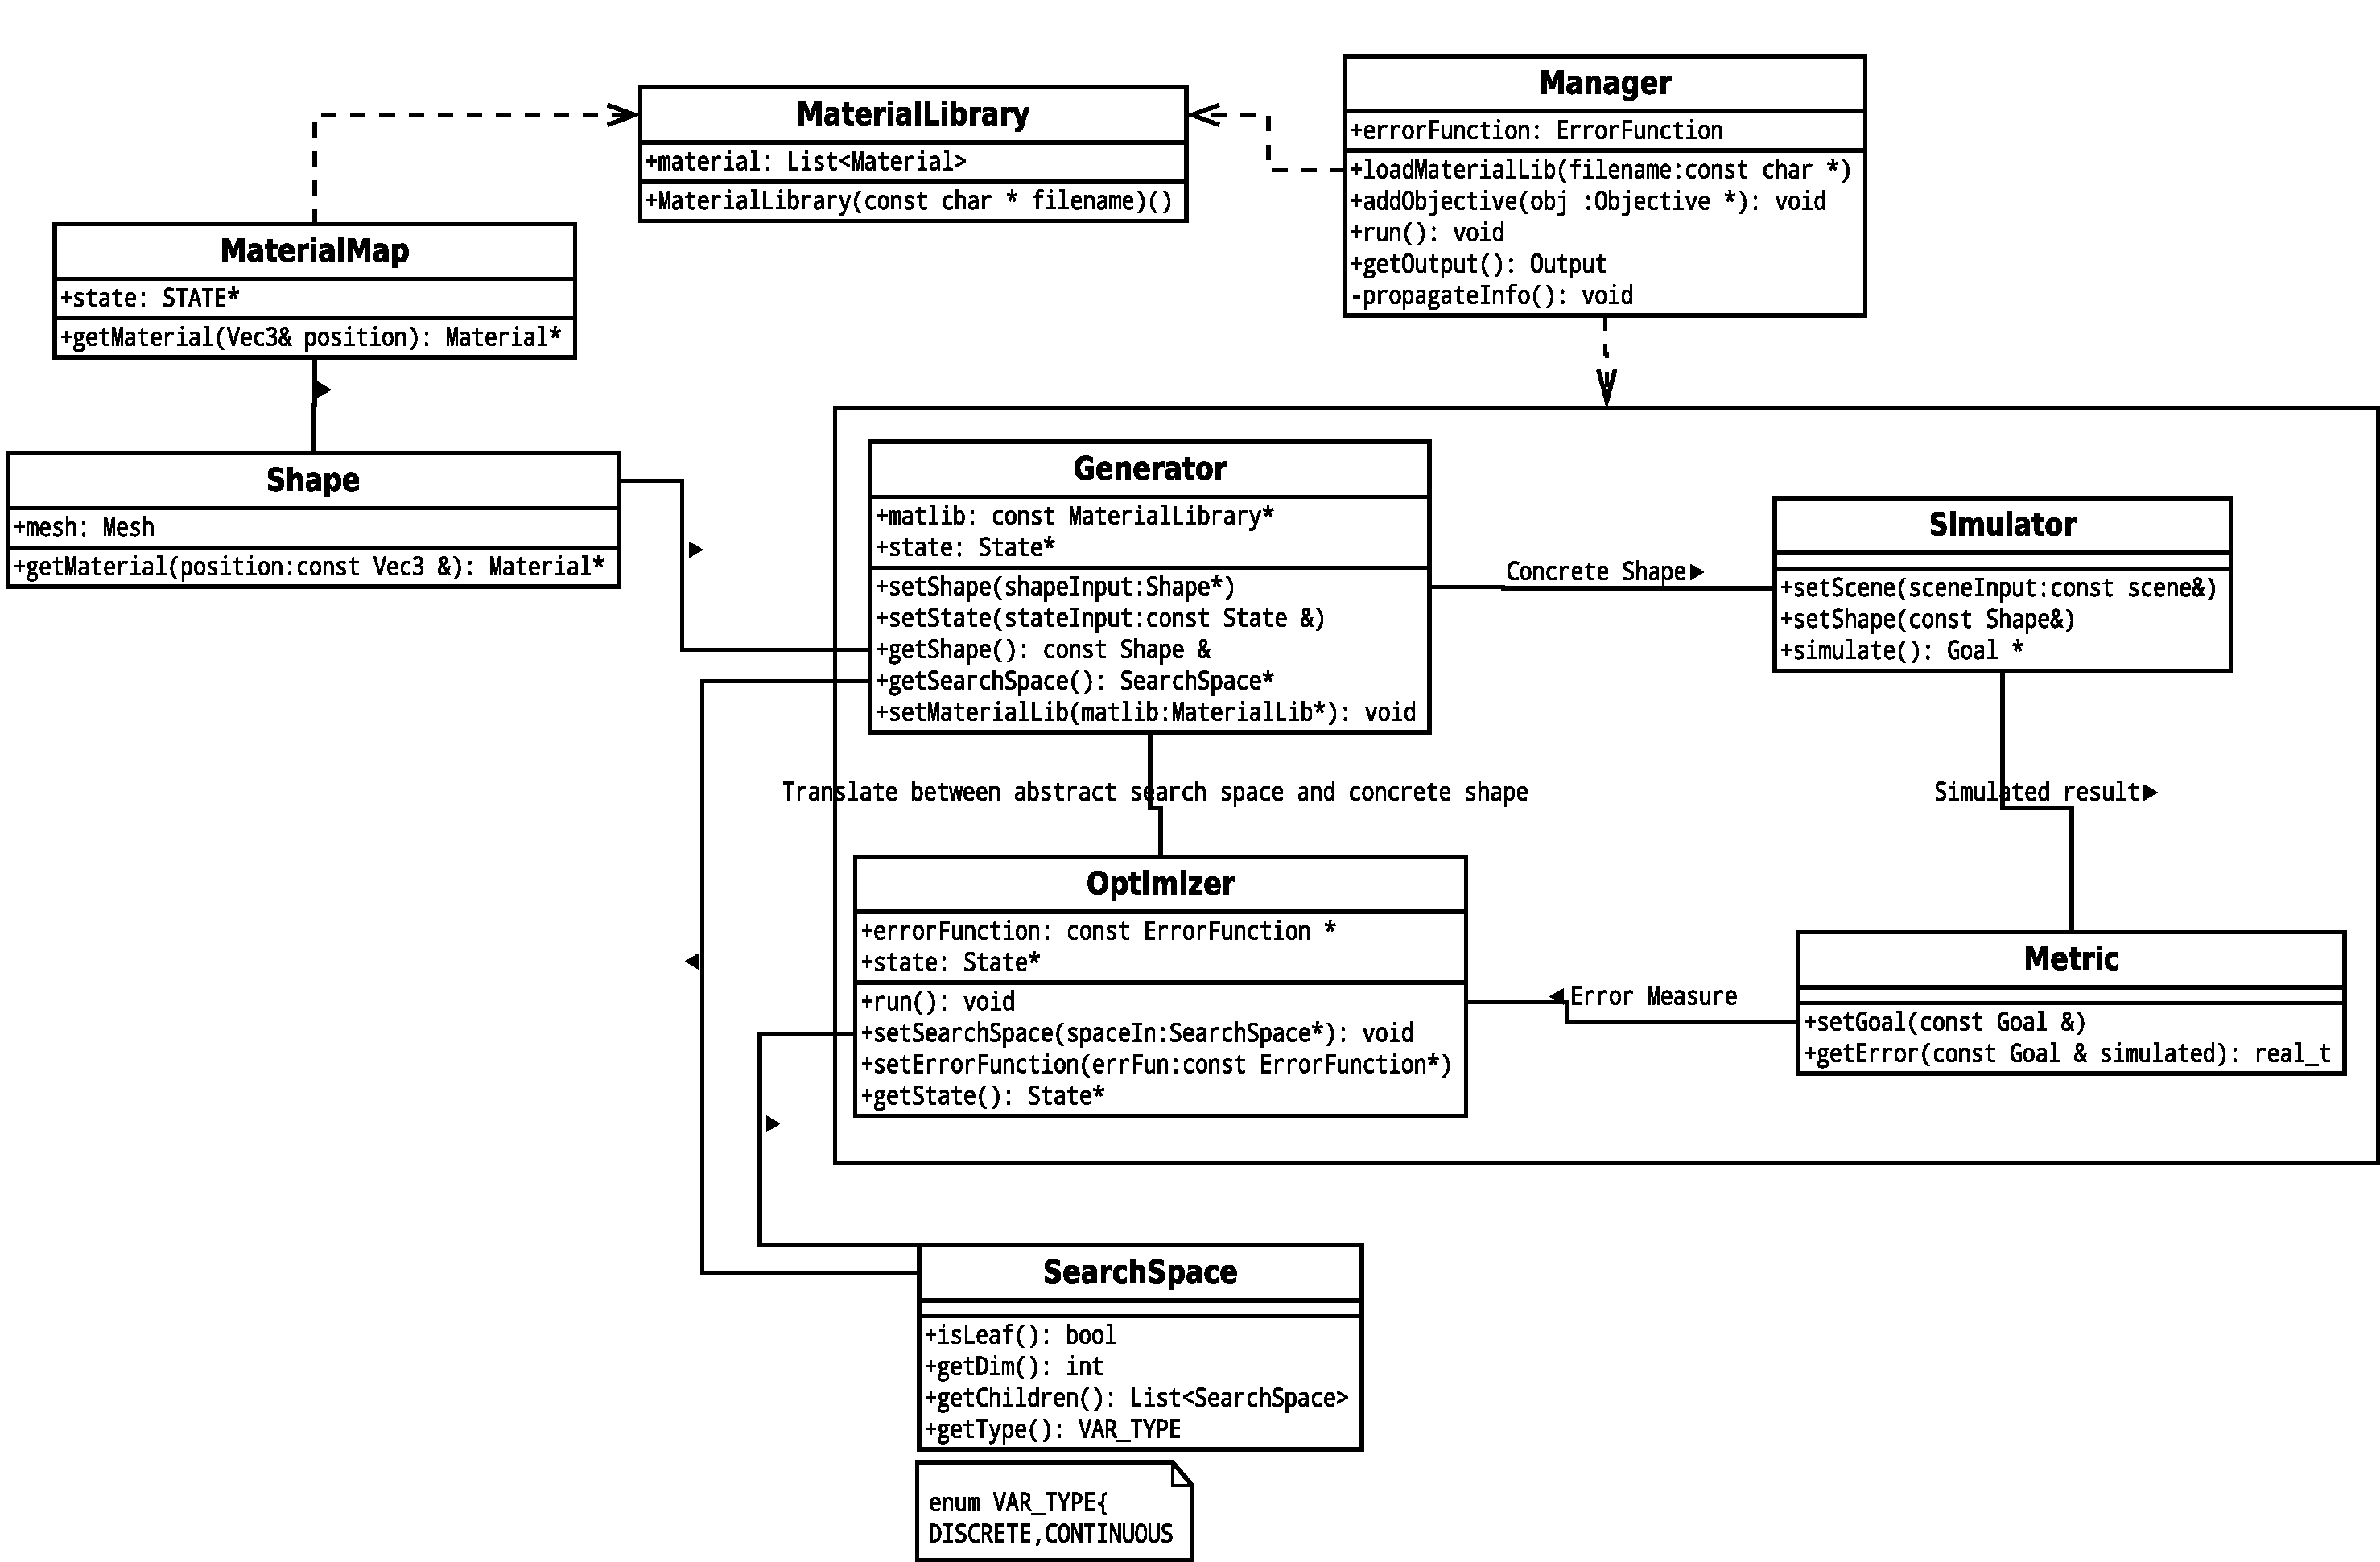
\includegraphics[width=0.45\textwidth]{figure/framework.pdf}
%\caption{API overview. The diagram will become nicer.}
%\label{fig:framework}
%\end{figure}
%\subsection{Input API}
%Our input API handles three tasks: specifying an optimization problem,
%maintaining a material library and configuring existing modules of
%the optimization process.
%An overview of the three components of our API is shown in Figure~\ref{fig:inputAPI}
%
%\begin{figure}
%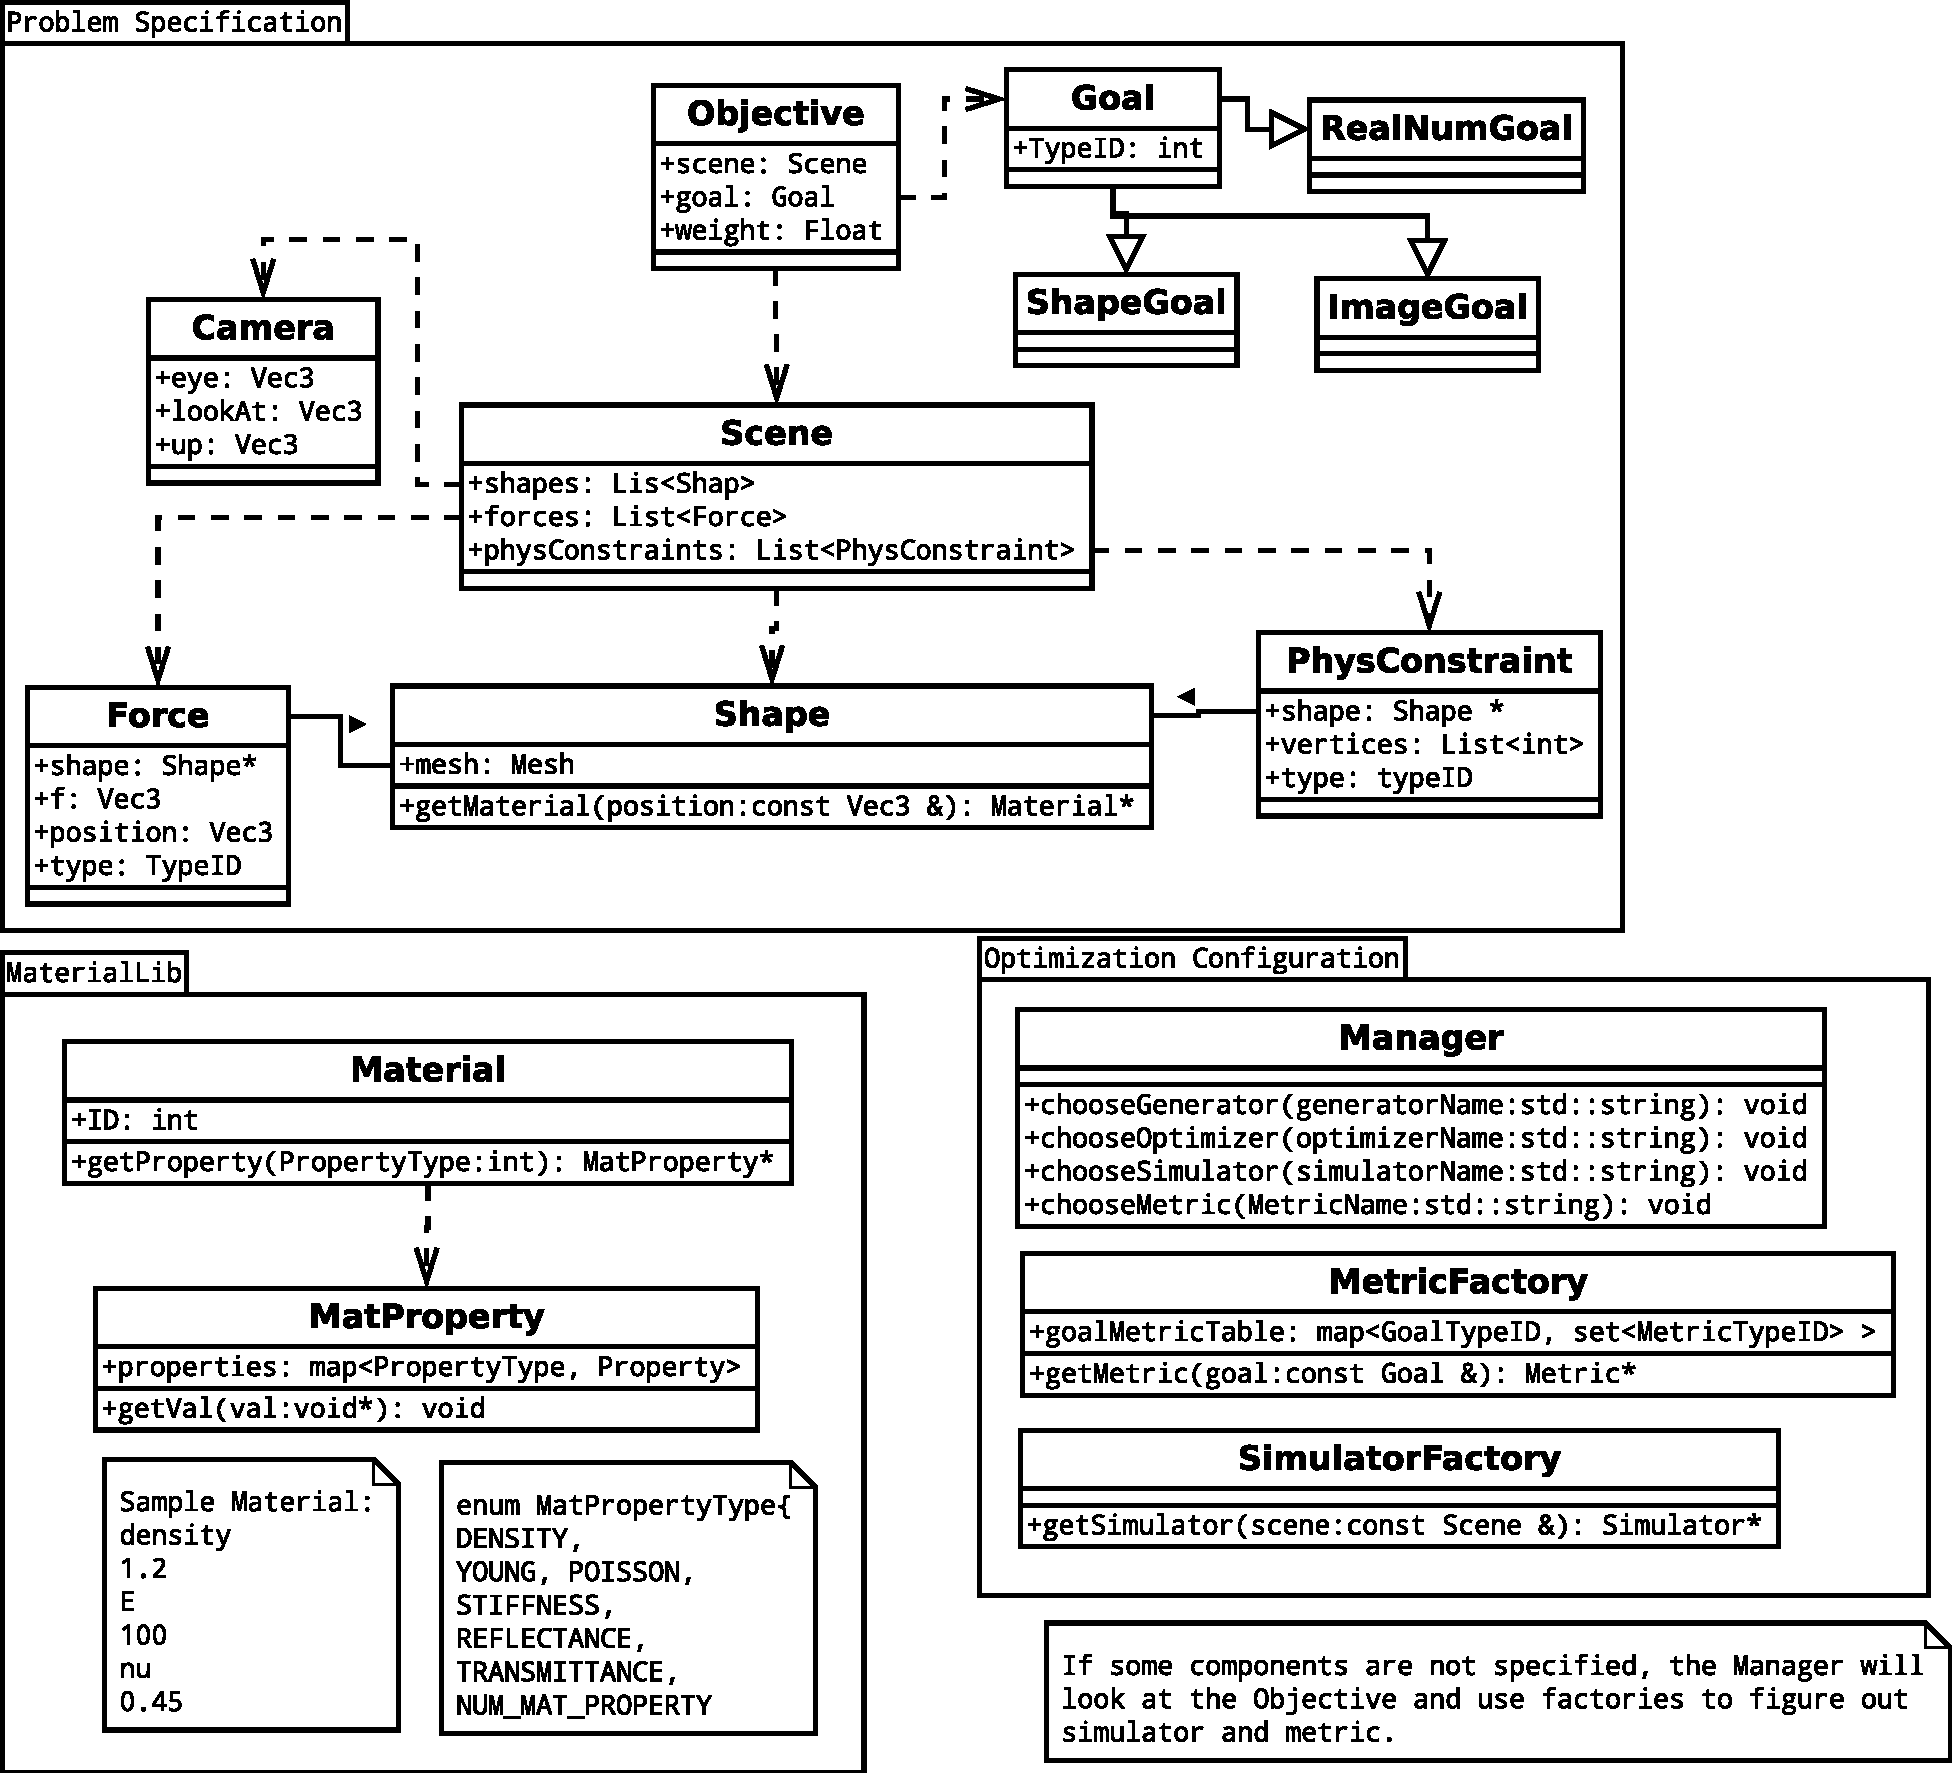
\includegraphics[width=0.45\textwidth]{figure/inputAPI.pdf}
%\caption{Input API. The diagram will become nicer.}
%\label{fig:inputAPI}
%\end{figure}
%
%Our input API allows a designer to either
%define material properties for sections of an object
%or specify behavior of an object.
%The designer
%can use functions to describe properties such as reflectance (e.g., BRDFs, BSSRDFs), 
%stiffness, or other spatially varying properties. 
%Although it is possible to define the object directly by only specifying material
%properties, intuitive user
%interfaces will aid in specifying the objects and their properties
%in terms of intuitive metaphors.
%For example, the elastic properties of an object can be specified by a set of
%example displacements from the rest pose and the corresponding applied forces.
%\subsection{Search Space Decomposition and Reduction}
%Our framework includes an optimization component that
%searches through the space of possible device inputs
%to find the one that best reproduces
%the desired object. Unfortunately, this search space
%is usually intractable. For example, when the printing
%volume has N voxels and each of these voxels can be
%assigned to one of M base materials, the search space
%contains $N^M$ choices. 
%To overcome this problem, we decompose the search
%space into similar subproblems and also reduce
%the search space to a lower-dimensional space using a reduction model. 
%The goal of the reduction step is to
%shrink the search space as much as possible but at the
%same time not to prune out good solutions. The low-dimensional space produced by the
%reducer can be defined in two different ways. First, a reduction model can be explicitly specified by an expert, for
%example, by defining structures of base materials and rules how different base materials can be combined together.
%In this paper, all reduction models are manually specified by us.
%The second way to specify a reduction model is implicit. In this case, the user provides a set of examples of
%valid material structures. Then, a machine learning algorithm infers both basic material structures and the rules
%for combining them. The optimization framework can be further improved by employing techniques that cluster
%partial solutions that yield similar output properties, avoiding combinatorial explosion of the search space.
%Furthermore, we can employ bounds on the solution based on physical constraints of the base materials.
%\subsection{Optimization}
%Our optimization component is an interface to
%existing standard optimization techniques
%such as simulated annealing, variational inference and
%Markov Chain Monte Carlo methods,
%as well as custom optimization algorithms implemented
%by more advanced users.
%\subsection{Simulation}
%Another key step in the process of converting abstractions to physical output is being able to
%simulate what an output device is going to generate given a well-defined input. 
%A simulation allows the user to preview how the output will look and behave. 
%This simulation is a generalization of the print-preview function
%available in word processing applications.
%As physical output generation might be costly or time-consuming, 
%it is extremely beneficial for users to be able to preview the output and make immediate changes to the design.
%That means that the simulation must accurately predict the output. 
%It's necessary to develop very efficient and accurate rendering
%and finite element simulation packages. Since we run the simulation multiple times within the optimization method
%we can cache and reuse partial simulation results, speeding up the evaluation process at least 10-100 times.
%Furthermore, we will ensure that the simulation is accurate by measuring properties of the printing materials and using
%these measurements to estimate the parameters of data-driven material models (e.g., for elasticity, reflectance).
%
%\section{Built-in Components}
%We provide a built-in library that handles common tasks such as assigning texture,
%simulating deformation, and optimizing for a stacking.
%\subsection{Generator}
%Generator uses a reduced representation
%of material assignments.
%Each generator is defined over a domain in the input shape.
%We provide a few basic generators and a composition operator.
%Let the input shape be over a domain $\Omega$.
%The composition of two generators $G_2\circ G_1$ is implemented by
%first letting $G_1$ reduce over a domain $\Omega_1$ and
%then letting $G_2$ reduce $\Omega_2 = \Omega-\Omega_1$.
%An example is shown in Figure~\ref{fig:genCompose}
%\begin{figure}[h]
%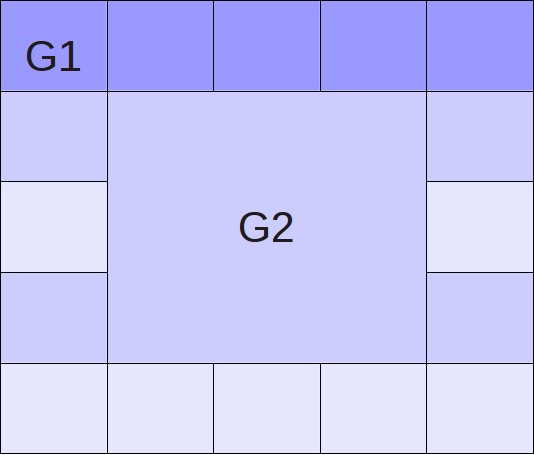
\includegraphics[scale=0.2]{figure/genCompose.png}
%\caption{Composition of two generators. $G_1$ is a fine-grained
%surface voxelization and $G_2$ is a very coarse inner
%grid.}
%\label{fig:genCompose}
%\end{figure}
%
%We will provide the following generators.
%\begin{enumerate}
%\item A generator that uses a uniform grids with homogeneous
%material in each grid cell. (A foam structure is treated as one homogeneous material).
%\item A generator that decomposes a mesh into columns of stackings.
%\item A polynomial spline for outline of a material.
%\end{enumerate}
%We use composition of the above basic generators to make the examples in 
%the result section.
%\subsection{Simulator}
%\begin{enumerate}
%\item Physics simulator with FEM, rigid body simulation
%and simple collision resolution.
%\item nVidia optiX to do photon mapping for caustics. Maybe also BRDF and shadows.
%We need to look at its speed.
%\item local computations such as reflectance and local mechanical properties given a stacking.
%\end{enumerate}
%
%\subsection{Metric}
%Optionally returns a gradient represented as an array of signed floats.
%\begin{enumerate}
%\item Compare a mesh and its deformed state. There is one-to-one correspondence of 
%vertices.
%\item compare two images
%\item compare two real numbers such as weight and bouncing height.
%\end{enumerate}
%
%\subsection{Optimizer}
%\begin{enumerate}
%\item MCMC, Simulated Anealing, SPSA
%\item Branch and bound (plus clustering of similar configurations)
%\item (Optional) reinforcement learning, deep neural networks...
%\end{enumerate}
%
%\section{Programming with Our API}
%A casual user mostly make function calls to an existing 
%manager to pass data and to run the optimization.
%More advanced user can configure the manager to achieve more specific requirements.
%For example, he can swap out an existing optimization module to achieve a better accuracy or 
%a faster speed.
%A professional user can implement more modules when he wants to deal with new
%material properties that are not handled by our built-in library. In that case,
%he needs to know what value the new property is in print materials, he needs to know
%how to simulate for the new property, and how to measure error of the new property.
%
%In below, we provide code snippets that handles three common tasks
%that we expect a moderately advanced user would write.
%
%Code examples:
%To generate textured model:
%\begin{verbatim}
%Manager manager;
%manager.loadMaterialLib("material_file");
%manager.setGenerator(
%  new HeightFieldGenerator());
%manager.setSimulator(colorSimulator());
%manager.setMetric(someColorMetric());
%manager.setOptimizer(
%  simulatedAnealing);
%  //or e.g. gradientDescent
%Objective obj;
%Scene scene;
%TexturedShape shape("filename");
%TexturedShape goal("filename1");
%scene.addShape(shape);
%obj.setScene(scene);
%obj.setGoal(goal);
%manager.addObjective(obj);
%\end{verbatim}
%
%To optimize BRDF for a particular camera view point and lighting.
%\begin{verbatim}
%scene.setCamera(camera);
%scene.addLight(light);
%manager.setGenerator(stackingGenerator);
%manager.setSimulator(brdfSimulator);
%manager.setMetric(someImageMetric);
%Shape shape("filename"), 
%Image goal("filename1");
%\end{verbatim}
%
%Defining elasticity properties
%by specifying deformation 
%reaction to a force applied to a point.
%
%\begin{verbatim}
%force = new Force(pos, dir, shapeID);
%constraint = new Constraint(
%    FIX_VERTEX, vertexList, shapeID));
%
%scene.addForce(force);
%scene.addConstraint(constraint);
%Shape goal;
%manager.setSimulator(femSimulator);
%\end{verbatim}

\note{I think we should just go with the results we have, texture etc... show the reducer network, tuner network, simulated results and manufactured result (if you have them}
\section{Results}
We used various generators in our experiments.
\subsection{Print Material Characterization and Measurement}
\subsection{Subsurface Scattering, Deformation and Mass}
Combining previous work on replicating
subsurface scattering and deformation behavior, 
we produced
material with a particular
look and deformation properties as shown in Figure~\ref{fig:deform}.
We als considered one additional property:mass. 
In this example, we
tried to make the material as light as possible.

We tried different combinations of generators in this experiment.
We compared the performance of these different generator
in terms of run-time and error.
\begin{enumerate}
\item Spline for top layer, fine-grained voxelization for mid layer
and a coarse grid for bottom layer.
\item Voxels for top layer, splines for middle layer and a coarse
bottom layer.
\item Find-grained voxels for top layer and coarse grid for bottom layer.
\end{enumerate}

\begin{figure}
\begin{subfigure}[b]{0.3\textwidth}
	\centering
 	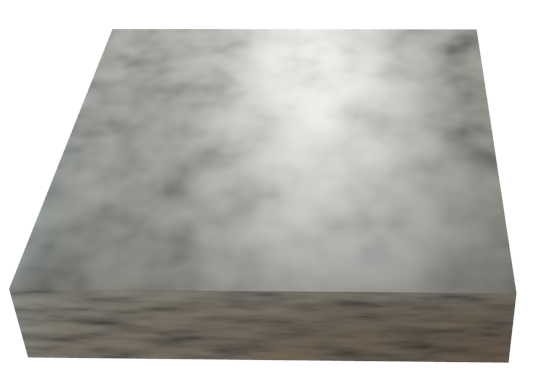
\includegraphics[width=\textwidth]{figure/slab_origin.png}
   	\caption{}
    \label{fig:deformPhoto}
    \end{subfigure}
    ~ 
    \begin{subfigure}[b]{0.3\textwidth}
    \centering
  	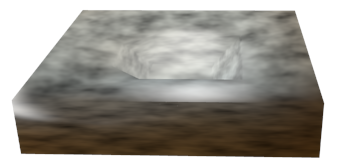
\includegraphics[width=\textwidth]{figure/slab_deform.png}
    \caption{}
    \label{fig:deformPrint}
\end{subfigure}
\caption{Simutaneously matching appearance and deformation. 
(a)Original slab of a particular looking. (b)printed slab 
with the same looking and desired deformation.}
\label{fig:deform}
\end{figure}

Two error plots showing subsurface scattering and deformation errors decrease
after each iteration in Figure~\ref{fig:err}.

\begin{figure}
\begin{subfigure}[b]{0.3\textwidth}
	\centering
 	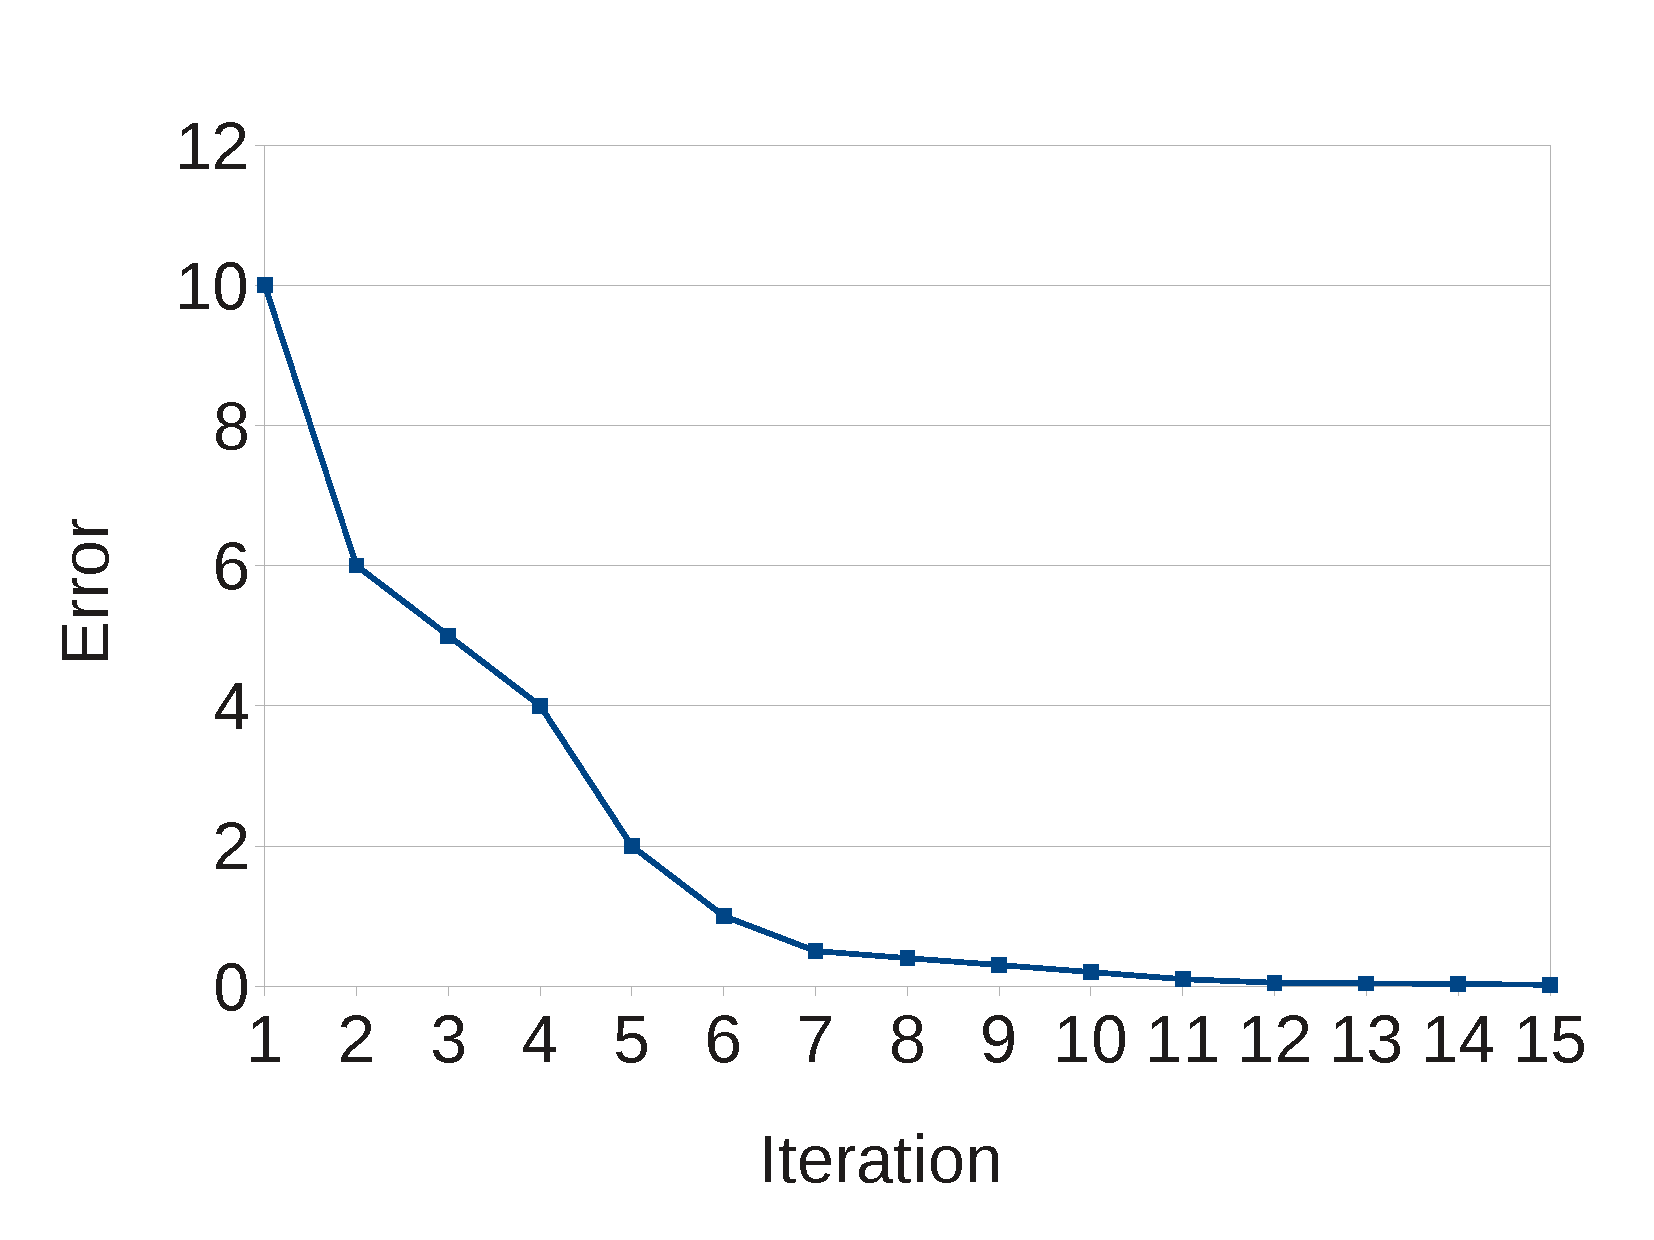
\includegraphics[width=\textwidth]{figure/error.pdf}
   	\caption{}
    \label{fig:ssErr}
    \end{subfigure}
    ~ 
    \begin{subfigure}[b]{0.3\textwidth}
    \centering
  	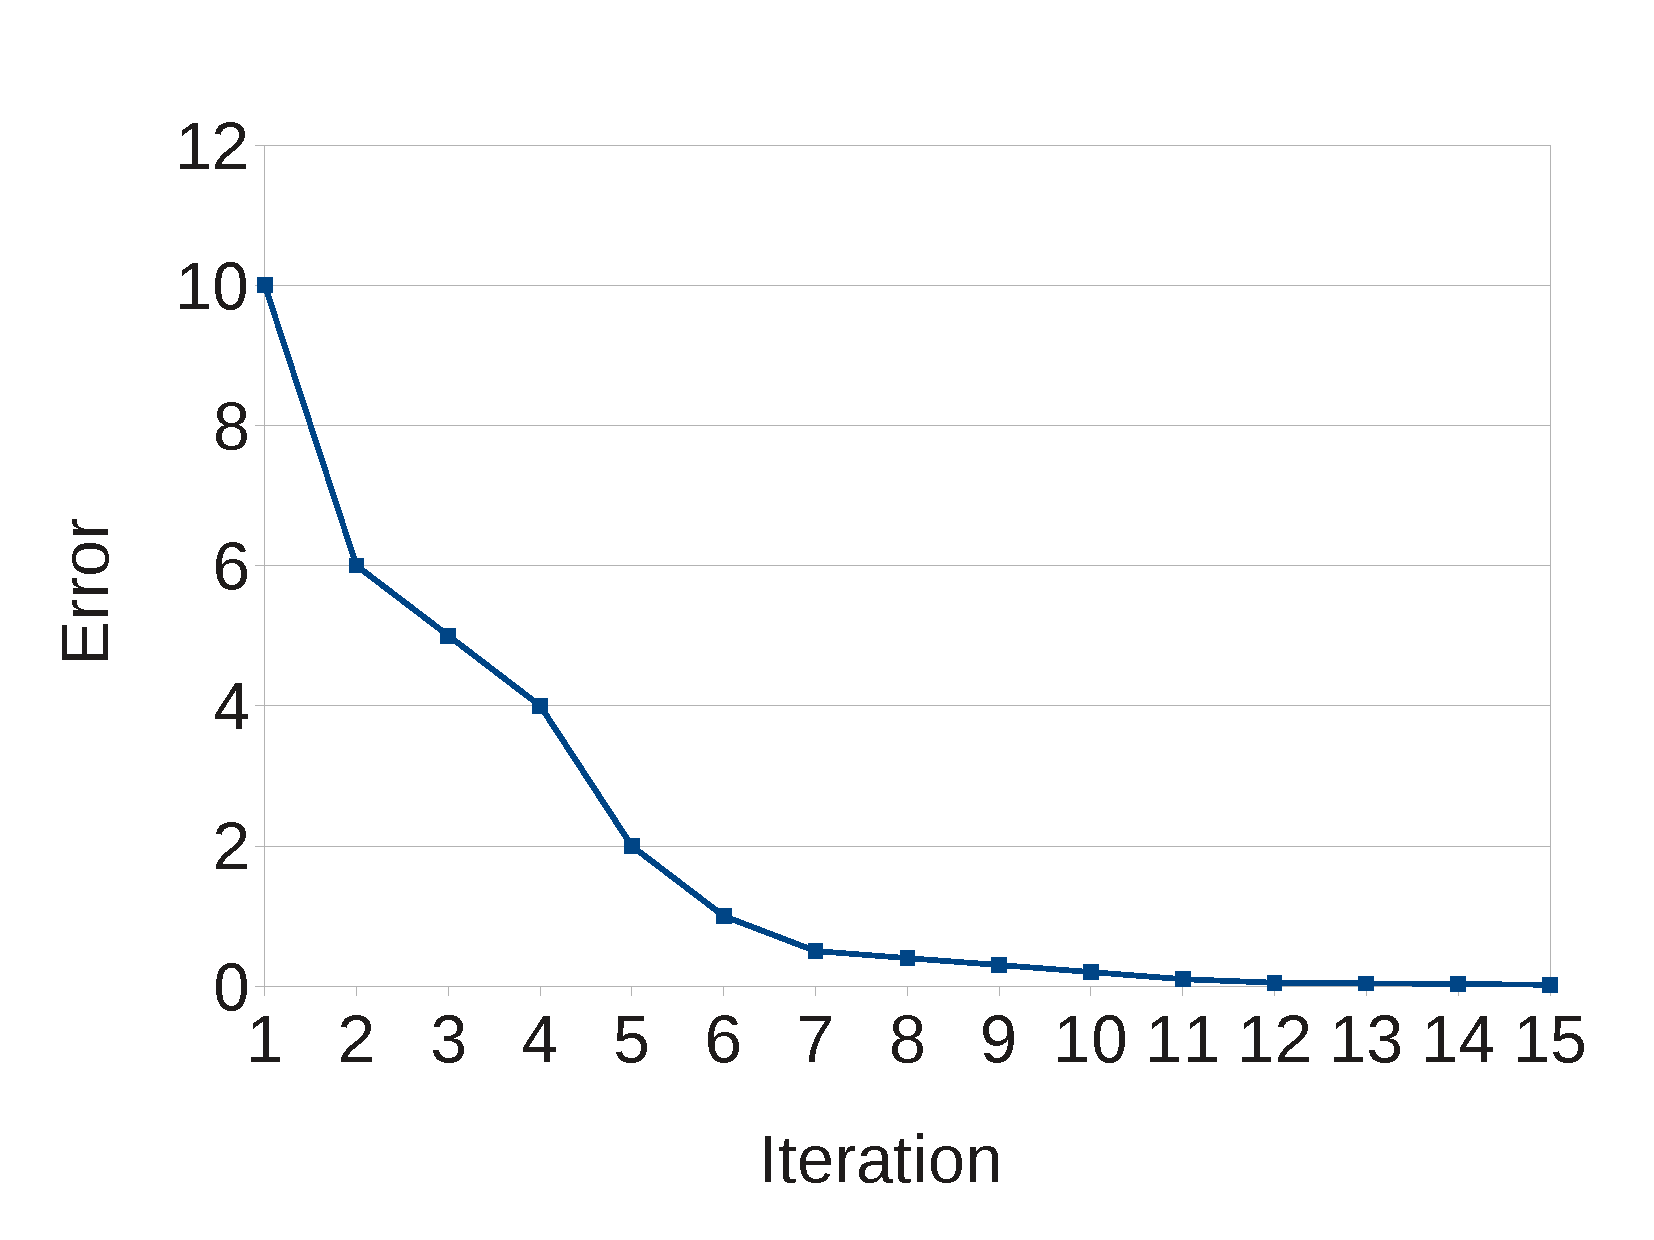
\includegraphics[width=\textwidth]{figure/error.pdf}
    \caption{}
    \label{fig:deformErr}
\end{subfigure}
\caption{Error plots for 
optimizing subsurface-scattering and deformation properties 
iteratively. (a)Subsurface scattering errors. (b)Deformation errors.}
\label{fig:err}
\end{figure}

\subsection{Caustics for a Mesh}
We demonstrate how to produce a 3D model with specific caustic shape under a particular lighting,
similar to \cite{Finckh:2010}. The difference is that we optimize on an arbitrary 3D model,
and we use a generic rendering package (NVidia optiX). 
We represented the surface with a spline surface.
Our algorithm took 6 hours to finish
with $4000$ spline control points for the model and $600\times 600$ resolution for the caustic image. A 
picture of our printed result under desired lighting is shown in Figure~\ref{fig:caustic}.

\begin{figure}
	\centering
 	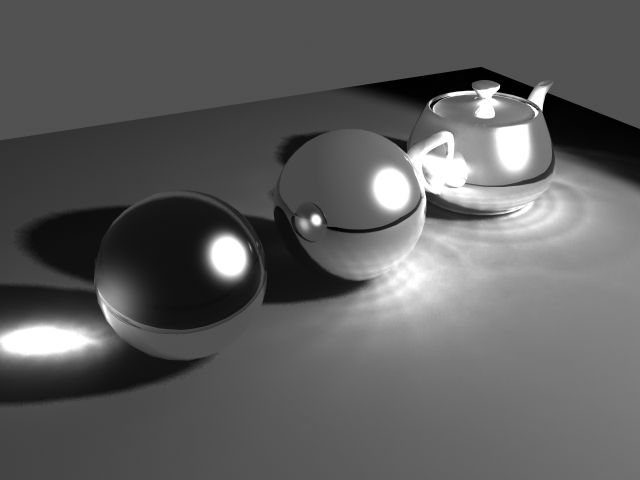
\includegraphics[width=0.3\textwidth]{figure/caustic.jpg}
\caption{Teapot with a caustic image.}
\label{fig:caustic}
\end{figure}

\subsection{Textured Model}
Input: a textured 3D model and
measured Albedo of print material.

Output: (Probably gray-scale) Material arranged for different printers in different formats: STL, fable,Gcode.

Printers: Our printer, Makerbot, Objet, maybe Zcorp.

When printing texture, only the outer layer matters. We used 
a composition of two generators: a very high resolution grid
for the outer layer and a uniform material for the inside.

We expand the set of printable colors by stacking translucent materials. We then applied
dithering with our expanded colors.
Results are shown in Figure~\ref{fig:texture}
\subsection{New Examples for Mechanical Properties}
Ball bounce to certain height. We used a higher resolution
grid for the out layer and very low resolution
for the inner mesh.

A plot of bounce height after each iteration.
The height and desired height is plotted in Figure~\ref{fig:ball}
\begin{figure}
	\centering
 	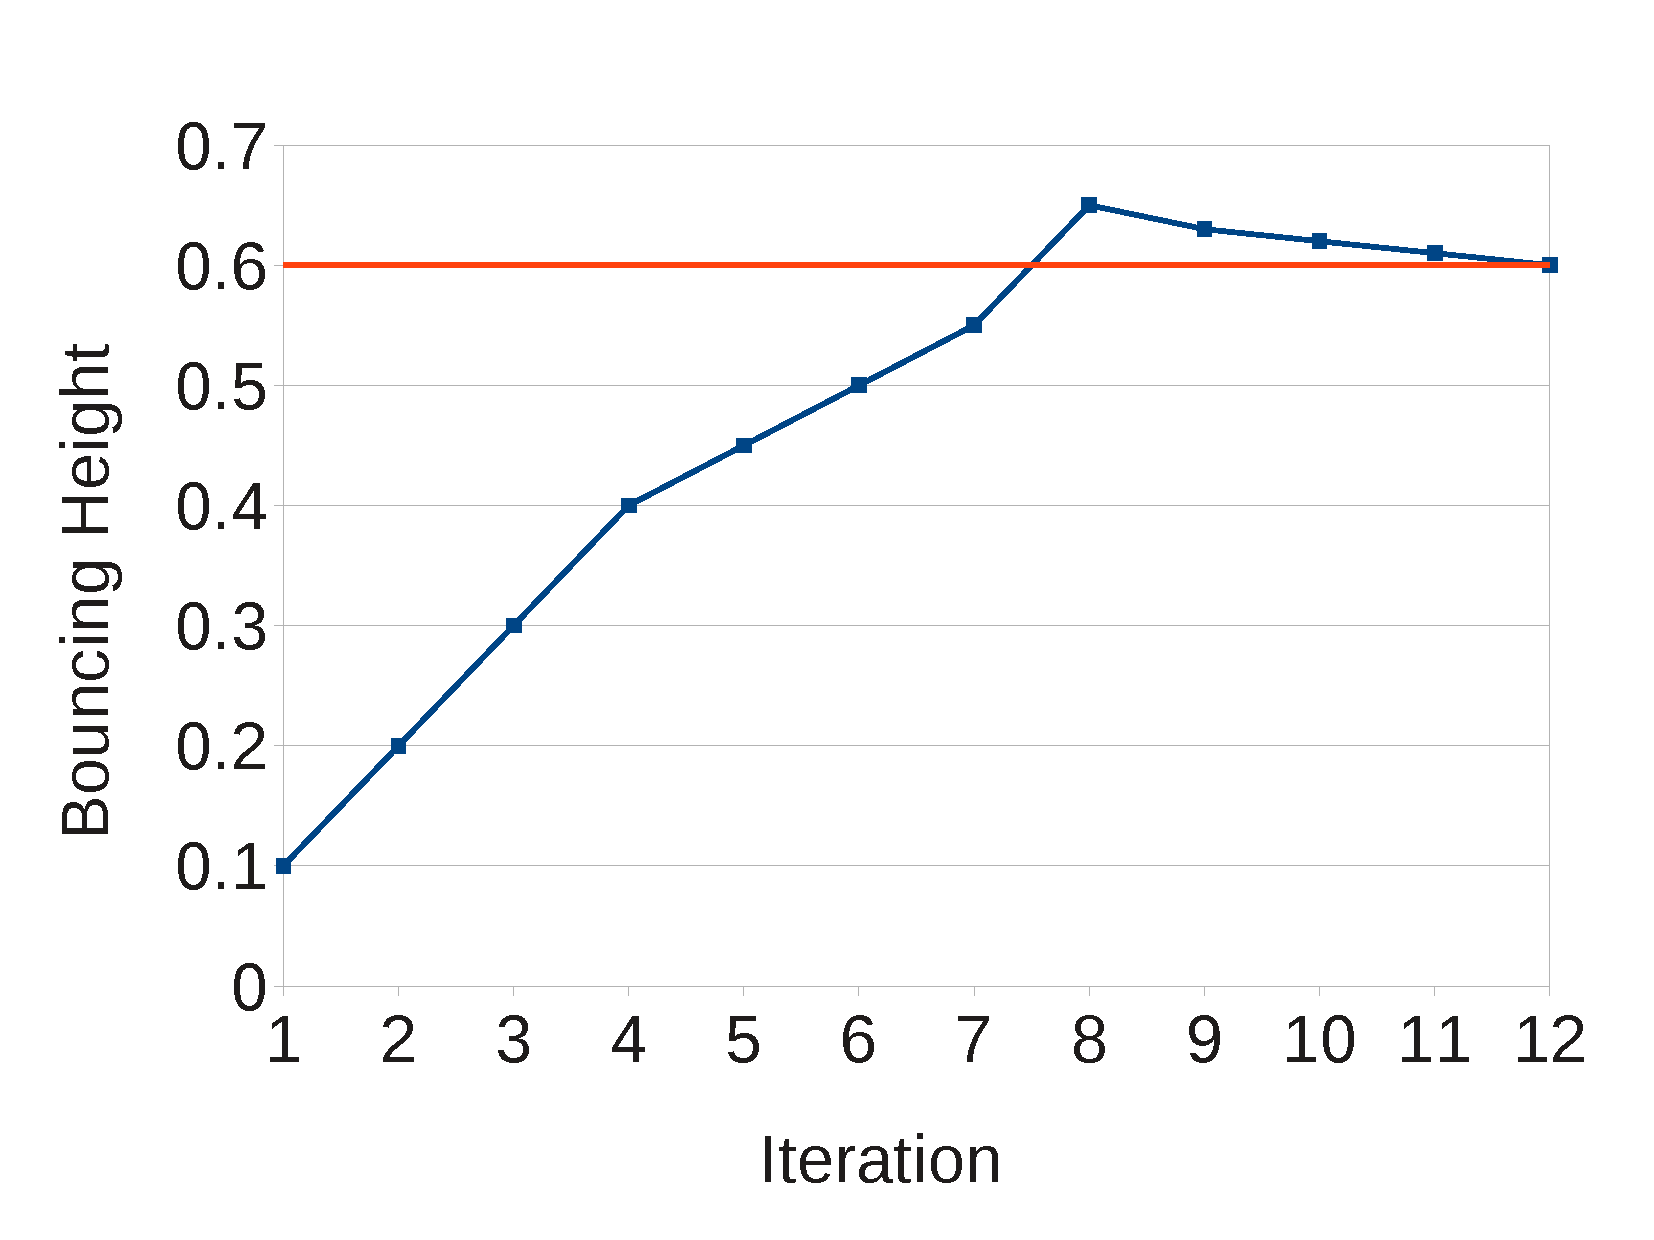
\includegraphics[width=0.3\textwidth]{figure/ballHeight.pdf}
\caption{Simulated height per-iteration of a ball bouncing after free-falling at 1 meter height.
	Redline is desired height.}
\label{fig:ball}
\end{figure}


A loaded die as shown in Figure~\ref{fig:die}. This example is interesting because
a local change will have some global effect.
We used very high resolution grid for the surface to match texture
of a die. The inner lay has only $3\times 3$ resolution.
\begin{figure}
	\centering
 	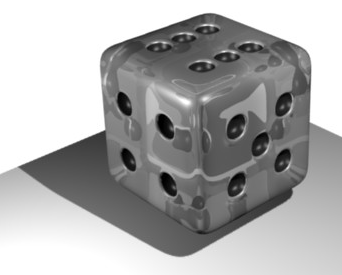
\includegraphics[width=0.25\textwidth]{figure/die.png}
\caption{A printed loaded die}
\label{fig:die}
\end{figure}
It has a certain probability to land on "1".
A table of probability distribution of landing on each side
is shown in Table~\ref{tab:dice}.

\begin{table}
\centering
  \begin{tabular}{ |c| p{0.7in} | p{0.7in} | }
  \hline
  face & simulated probability & measured probability\\
  \hline
  1 & 0.5 & 0.5\\
  \hline
  2 & 0.1 & 0.1\\
  \hline
  3 & 0.1 & 0.1\\
  \hline
  4 & 0.1 & 0.1\\
  \hline
  5 & 0.1 & 0.1\\
  \hline
  6 & 0.1 & 0.1\\

  \hline
  \end{tabular}
  \caption{Simulated and measured dice probability}
  \label{tab:dice}
\end{table}

A plot of simulated probability of landing on "1" after each iteration
is shown in Figure~\ref{fig:dieErr}.

\begin{figure}
	\centering
 	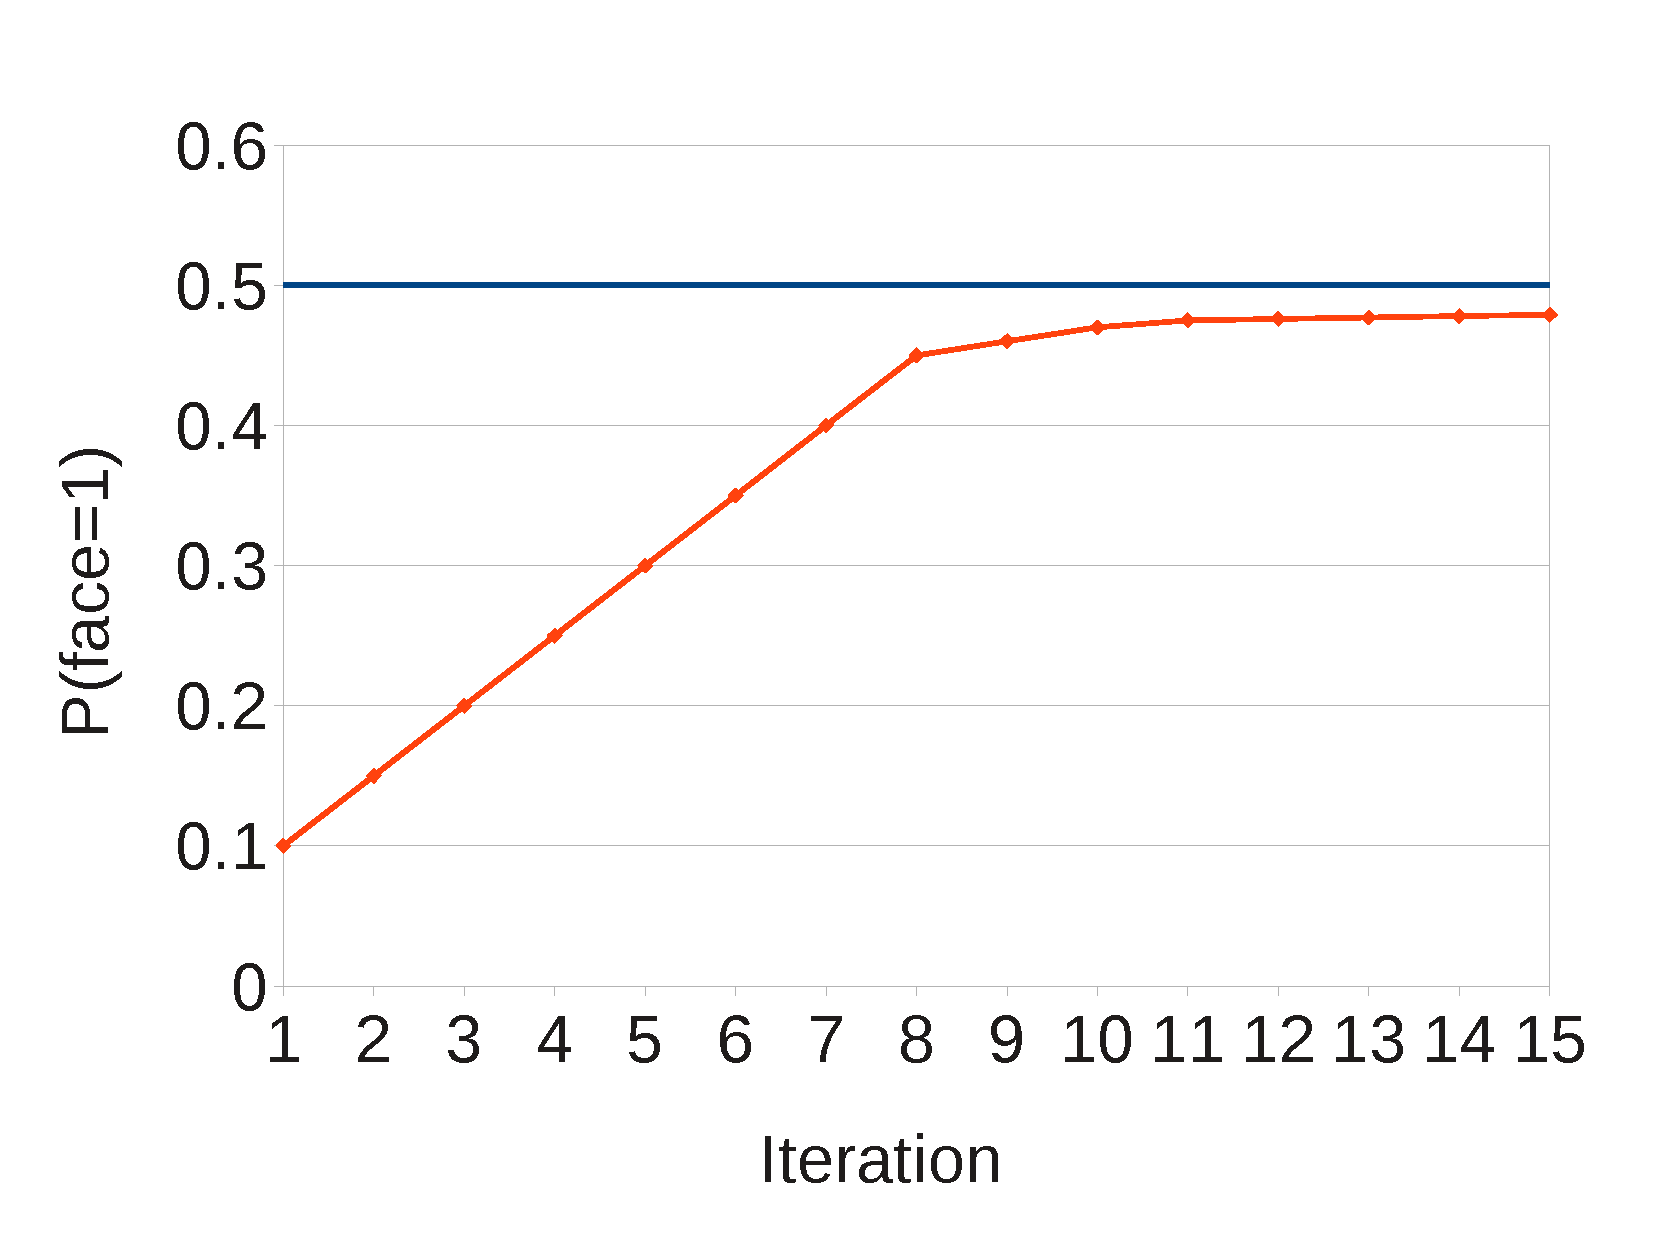
\includegraphics[width=0.3\textwidth]{figure/die.pdf}
\caption{Probability of die landing on 1 after each iteration.}
\label{fig:dieErr}
\end{figure}

Printer:objet, ours.

More ideas:
balancing bird with texture.
\section{Possible Extension}
UI to specify input deformation.
\section{Conclusion}
\section*{Acknowledgements}

\bibliographystyle{acmsiggraph}
\bibliography{paper}
\end{document}
